\documentclass[mathserif, aspectratio=169]{beamer}
\usetheme{odenpecos}
\setbeamertemplate{itemize/enumerate body begin}{\fontsize{8.8}{9}\selectfont}
\setbeamertemplate{itemize/enumerate subbody begin}{\fontsize{7.5}{8}\selectfont}
\setbeamertemplate{itemize/enumerate subsubbody begin}{\fontsize{7.5}{8}\selectfont}

% default search path for figures
\graphicspath{{./../fig/}}

\newcommand{\zapspace}{\topsep=0pt\partopsep=0pt\itemsep=0pt\parskip=0pt}

\usepackage{multicol}
\usepackage{multirow}
\usepackage{pict2e}
%\usepackage{esdiff}
\usepackage{multimedia}
\usepackage{verbatim}
\usepackage{mhchem}
\usepackage{tikz}
\usetikzlibrary{arrows}
\usepackage[percent]{overpic}
\usepackage[absolute,overlay]{textpos}
\usepackage{tikz} % Required for flow chart
\usepackage[caption=false]{subfig}
\usepackage{pgfplots}

\newcommand{\overbar}[1]{\mkern 1.5mu\overline{\mkern-1.5mu#1\mkern-1.5mu}\mkern 1.5mu}
\newcommand{\pp}[2]{\frac{\partial #1}{\partial #2}}
\newcommand{\dd}[2]{\frac{d #1}{d #2}}
\newcommand{\DD}[2]{\frac{D #1}{D #2}}
\newcommand{\mm}{\mathbf{minmod}}
\def\etal{{\it et al~}}
\newcommand{\be}{\begin{eqnarray}}
	\newcommand{\ee}{\end{eqnarray}}
\newcommand{\mbb}[1]{\mathbb{#1}} % math blackboard bold
\newcommand{\mcal}[1]{\mathcal{#1}} % math blackboard bold
\newcommand{\mbf}[1]{\mathbf{#1}} % math bold face (for vectors)
\newcommand{\sbf}[1]{\boldsymbol{#1}} % bold face for symbols
\newcommand{\jump}[1]{\llbracket #1 \rrbracket} % jump operator
\newcommand{\avg}[1]{\langle #1 \rangle} % average operator
\newcommand{\rarrow}{\rightarrow}
\newcommand{\Rarrow}{\Rightarrow}
\newcommand{\LRarrow}{\Leftrightarrow}
\newcommand{\vvvert}{|\kern-1pt|\kern-1pt|}
\newcommand{\enorm}[1]{\vvvert #1 \vvvert}
\newcommand{\nutil}{\tilde{\nu}}
\newcommand{\Var}{\mathrm{Var}}
\newcommand{\Cov}{\mathrm{Cov}}


\definecolor{MyDarkGreen}{rgb}{0,0.45,0.08}
\newcommand{\myred}[1]{{\color{red} #1}}
\newcommand{\myblue}[1]{{\color{blue} #1}}
\newcommand{\mygreen}[1]{{\color{MyDarkGreen} #1}}

\newcommand{\sa}{\nu_{\mathrm{sa}}}
\newcommand{\tep}{\tilde{\epsilon}}
\newcommand{\Ssd}{\mathcal{S}} % source term due to slow derivative
\newcommand{\ud}{\,\mathrm{d}}

\newcommand{\Mach}[1]{\ensuremath{\mbox{Ma}_{#1}}}
\newcommand{\Reynolds}{\ensuremath{\mathit{Re}}}
\newcommand{\DensityRat}{\ensuremath{\mathit{DR}}}
\newcommand{\BlowRat}{\ensuremath{\mbox{BR}}}
\newcommand{\VelRat}{\ensuremath{\mathit{VR}}}
\newcommand{\Tau}{\ensuremath{\mathrm{T}}}

\newcommand{\wall}     {\ensuremath{\mathrm{w}}}   % wall subindex
\newcommand{\awall}    {\ensuremath{\mathrm{aw}}}  % adiabatic wall subindex

\newcommand{\commentout}[1]{}

\newcommand{\vect}[1]{\boldsymbol{#1}}
\usepackage{mleftright}
\newcommand{\of}[1]{\mleft( #1 \mright)}
\newcommand{\vth}{v_{\textrm{th}}}
\newcommand{\reals}{\mathbb{R}}
\newcommand{\myint}{\int\limits}
\newcommand{\ddt}[1]{\partial_t #1}
\newcommand{\RR}{\mathbb{R}}
\newcommand{\vr}{v}
\newcommand{\diff}[1]{\, d#1}
\newcommand{\norm}[1]{\left\lVert#1\right\rVert}
%\newcommand{\vtheta}{\theta_{\vect{v}}}
%\newcommand{\vphi}{\varphi_{\vect{v}}}
%\newcommand{\vr}{v_{r}}
\newcommand{\vtheta}{{v_{\theta}}}
\newcommand{\vphi}{v_{\varphi}}
\newcommand{\vomega}{v_{\omega}}
\newcommand{\vrunit}{\hat{\vect{v}}_{r}}
\newcommand{\vthetaunit}{\hat{\vect{v}}_{\theta}}
\newcommand{\vphiunit}{\hat{\vect{v}}_{\varphi}}
\DeclareMathOperator{\variance}{Var}

\usepackage{mathtools}
\DeclarePairedDelimiter\ceil{\lceil}{\rceil}
\DeclarePairedDelimiter\floor{\lfloor}{\rfloor}
\usepackage{tikz}

\usepackage{tcolorbox}
\tcbuselibrary{minted,breakable,xparse,skins}
\definecolor{bg}{gray}{0.95}
\DeclareTCBListing{mintedbox}{O{}m!O{}}{%
	breakable=true,
	listing engine=minted,
	listing only,
	minted language=#2,
	minted style=default,
	minted options={%
		linenos,
		gobble=0,
		breaklines=true,
		breakafter=,
		fontsize=\small,
		numbersep=8pt,
		#1},
	boxsep=0pt,
	left skip=0pt,
	right skip=0pt,
	left=25pt,
	right=0pt,
	top=3pt,
	bottom=3pt,
	arc=5pt,
	leftrule=0pt,
	rightrule=0pt,
	bottomrule=2pt,
	toprule=2pt,
	colback=bg,
	colframe=orange!70,
	enhanced,
	overlay={%
		\begin{tcbclipinterior}
			\fill[orange!20!white] (frame.south west) rectangle ([xshift=20pt]frame.north west);
	\end{tcbclipinterior}},
	#3,
}

\begin{document}
% disable nav
\setbeamertemplate{navigation symbols}{}

% ---------------------------------------------------------------
% Oden/Pecos title page

\hoffset=.16in

\begin{frame}[plain,t]{}
\makeatletter
%\vspace*{0.85cm}
%\vspace*{0.65cm}
\includegraphics[height=0.9in,trim=50 40 40 0, clip]{PMSc_159_university_formal_horizontal.pdf} \newline
%\vspace*{0.3cm}
\begin{columns}[T,onlytextwidth]
\column{.8\textwidth}
{\bf \color{burntorange} \fontfamily{bch}\selectfont 
% -- Set talk title here
Integration efforts on the electron Boltzmann solver with the torch plasma simulator
%Electron Boltzmann solver integration with the torch plasma simulator
% --
}
\end{columns}
\vspace*{.15cm}
\rule{.8\textwidth}{0.6pt} \newline

\vspace*{0.05cm}
\setstretch{0.65}
{\fontfamily{phv}\selectfont
  { \scriptsize
    % -- define presenter, authors here
    Milinda Fernando, Kinetic solvers, Parla, and TPS team members \\
    % --
  }
  {\color{burntorange} \tiny
    % -- define role, meeting event, location, etc
    PSAAP III Annual Review $\cdot$ November 08-09, 2023
    %PSAAP TST Meeting $\cdot$ April 24-25, 2023
    % --
  }
}

\vspace*{1cm}
%\includegraphics[height=0.3in]{figures/pecos_orange1.png}
\begin{columns}
\begin{column}{0.8\linewidth}
\includegraphics[height=0.5in]{oden_pecos_2020_wordmark.png}\\
{\scriptsize \url{https://pecos.oden.utexas.edu}}
\end{column}

\begin{column}{0.2\linewidth}
\includegraphics[height=0.6in]{psaap3-logo.png}
\end{column}
\end{columns}

\end{frame}
\hoffset=0in
% -- end title slide ---------------------------------------------

%\begin{frame}
%	\frametitle{Outline}
%	\begin{itemize}
%		\item Spatially homogeneous Boltzmann equation, $\partial_t f - \frac{\vect{E} q}{m} \cdot \nabla_{\vect{v }}f = C(f)$
%		\item Representation of $f$ (i.e., isotropic + anisotropic correction terms), use spherical harmonics for angular directions + experimentation of basis functions in radial direction. 
%		\begin{itemize}
%			\item Global approximations with Maxwell and Laguerre polynomials.
%			\item Local approximations with linear and higher order B-splines
%		\end{itemize}
%		\item Collision operator (5d integral form)
%		\item Simplifications for the collision operator with analytical integration of angular directions (1d integral form). 
%		\item Equations for the steady-state solution (spatially homogeneous case) 
%		\item Two-term formulation vs. EEDF formulation with diffusion term. 
%		\item Verification with Bolsig+ code.  (Both approaches, importance of the diffusion term), PS 2.4
%		\item Formulation for 1D-space+3D-velocity space Boltzmann equations with some preliminary results for 1d glow discharge problem. 
%		\item Discuss on single GPU implementation with CuPy, Challenges in 1D+3V formulation (i.e., boundary conditions) and Future work, ES 2.6
%	\end{itemize}
%\end{frame}

\begin{frame}
	\frametitle{Where do we fit ?}
	\begin{figure}
		\centering
		\includegraphics[width=0.9\textwidth]{where_we_fit.png}
	\end{figure}
\end{frame}

%\begin{frame}
%	\frametitle{Outline}
%\end{frame}

\begin{frame}
	\frametitle{Torch plasma simulator}
	\begin{columns}
		\begin{column}{0.48\textwidth}
			\textbf{TPS with LTE}
			%\vspace{0.25in}
			\footnotesize
			\begin{align*}
				&\partial_t n_i + \nabla_{\vect{x}} \cdot \vect{J_{n_i}}  = k_i n_0 n_i  \color{gray}{\text{ in } \Omega_x \times (0,T]}\\
				%\partial_t n_0 + \nabla_{\vect{x}} \cdot \vect{J_{n_0}}  = -k_i n_0 n_i \text{ in } \Omega_x \times (0,T]\\
				&\text{conservation of mass, momentum} \\
				&\quad  \text{and energy for } \vect{u}, n_0, T_g \\
				%\text{conservation of momentum for }  r^{+}, Ar  \\
				&\text{Maxwell's equations for } \vect{E}
			\end{align*}
			\begin{itemize}
				\item LTE: $T_g=T_e$ %Assumes local thermodynamic equilibrium, (i.e., $T_e = T_g$) and quasi-neutrality (i.e., $n_e=n_i$)
				\item Quasi-neutrality: $n_e = n_i$ 
				\item $k_i \approx$ Maxwellian EEDF at $T_g$
			\end{itemize}
		\end{column}
		\begin{column}{0.48\textwidth}
			\textbf{TPS + Boltzmann}
			%\vspace{0.25in}
			\footnotesize
			\begin{align*}
				&\partial_t n_i + \nabla_{\vect{x}} \cdot \vect{J_{n_i}}  = k_i n_0 n_i  \color{gray}{\text{ in } \Omega_x \times (0,T]}\\
				%\partial_t n_0 + \nabla_{\vect{x}} \cdot \vect{J_{n_0}}  = -k_i n_0 n_i \text{ in } \Omega_x \times (0,T]\\
				&\text{conservation of mass, momentum} \\
				&\quad  \text{and energy for } \vect{u}, n_0, T_g \\
				%\text{conservation of momentum for }  r^{+}, Ar  \\
				&\text{Maxwell's equations for } \vect{E}\\
				&\partial_t f  + \vect{v} \cdot \nabla_{\vect{x}} f -\frac{\vect{E} q}{m} \cdot \nabla_{\vect{v }}f = C(f, n_0, T_g) \color{gray}{\text{ in } \Omega_x \times \Omega_v \times (0,T]}
			\end{align*}
			\begin{itemize}
				\item $T_e \sim \int_{\vect{v}} \norm{\vec{v}}^2 \hat{f} \diff{\vect{v}}$
				\item $k_i = \int_{\vect{v}} \sigma(\norm{\vect{v}}) \hat{f} \diff{\vect{v}}$ where $\hat{f} = \frac{f}{\int_{\vect{v}} f \diff{\vect{v}}}$
				%\item 7D problem
			\end{itemize}
		\end{column}
	\end{columns}

\end{frame}

\begin{frame}
	\frametitle{TPS + Boltzmann}
	% \begin{itemize}
	% 	\item Importance of spatially coupled Boltzmann on torch QoIs to be determined
	% 	\item Current approach: Batch of spatially homogeneous Boltzmann solves for the $\Omega_x$
	% \end{itemize}
	\vspace{0.2in}
	\begin{columns}
		\begin{column}{0.48\textwidth}
			\textbf{Strong coupling (2-way)}\\
			\begin{figure}
				\resizebox{0.9\textwidth}{!}{
					\centering
					\begin{tikzpicture}[block/.style={draw=black,thick, inner sep=2pt, rounded corners, minimum width=2cm, minimum height=1.2cm, fill=rightfooterorange,font={\small}}, shift=(current page.center)]
						\begin{scope}[yshift=10cm,xshift=5cm]
							% \draw[lightgray]
							% (current page.north) -- (current page.south)
							% (current page.west)  -- (current page.east);
							\node[block] (A) at (-9, 3) {TPS};
							\node[block] (C) at (-3 , 3.001) {Boltzmann};
							% \node[block] (D) at (0.002 , 0) {electron kinetic coefficients ($T_g, E/n_0, n_e/n_0, E$)};
							% \draw [->,very thick] (B) -- node [text width=3cm, midway, above, align=center,xshift =-0.8cm] {with Maxwellian assumption $f = M_{T_e}(\vect{v})$} (A);\pause
							% \draw [->,very thick] (B) -- node [text width=3cm, midway, above, align=center,xshift = 1.6cm, yshift=-0.5cm] {collision operator assembly} (C);
							% \draw [->,very thick] (C) -- node [text width=3cm, midway, above, align=center, yshift=-0.5cm, xshift=1.2cm] {static E-field assumption} (D);
							% \draw [->,very thick] (D) -- node [text width=3cm, midway, above, align=center,xshift =-1.2cm, yshift=-1.8cm] {$T_e$-based \\ interpolation for rates, kinetic coefficients} (A);\pause
							\draw [->,very thick] (A) to[bend left  = 8] node [text width=3cm, midway, above, align=center,yshift=0cm] {$T_g, E(x,t), n_e, n_0$} (C);
							\draw [->,very thick] (C) to[bend left  = 8] node [text width=3cm, midway, below, align=center,xshift=0.0cm] {$k_i$, $n_e$, $T_e$} (A);
						\end{scope}
				\end{tikzpicture}}
			\end{figure}
		\end{column}
		\begin{column}{0.48\textwidth}
			\textbf{Weak coupling (1-way)}\\
			\begin{figure}
				\resizebox{0.9\textwidth}{!}{
					\centering
					\begin{tikzpicture}[block/.style={draw=black,thick, inner sep=2pt, rounded corners, minimum width=2cm, minimum height=1.2cm, fill=rightfooterorange,font={\small}}, shift=(current page.center)]
						\begin{scope}[yshift=10cm,xshift=5cm]
							% \draw[lightgray]
							% (current page.north) -- (current page.south)
							% (current page.west)  -- (current page.east);
							\node[block] (A) at (-9, 3) {TPS};
							\node[block] (C) at (-3 , 3.001) {Boltzmann};
							\node[] (B) at (-9, 1.2) {$k_i^{tps}$};
							\node[] (D) at (-3, 1.2) {$k_i^{bte}$};

							% \node[block] (D) at (0.002 , 0) {electron kinetic coefficients ($T_g, E/n_0, n_e/n_0, E$)};
							% \draw [->,very thick] (B) -- node [text width=3cm, midway, above, align=center,xshift =-0.8cm] {with Maxwellian assumption $f = M_{T_e}(\vect{v})$} (A);\pause
							% \draw [->,very thick] (B) -- node [text width=3cm, midway, above, align=center,xshift = 1.6cm, yshift=-0.5cm] {collision operator assembly} (C);
							% \draw [->,very thick] (C) -- node [text width=3cm, midway, above, align=center, yshift=-0.5cm, xshift=1.2cm] {static E-field assumption} (D);
							% \draw [->,very thick] (D) -- node [text width=3cm, midway, above, align=center,xshift =-1.2cm, yshift=-1.8cm] {$T_e$-based \\ interpolation for rates, kinetic coefficients} (A);\pause
							\draw [->,very thick] (A) to[bend left  = 8] node [text width=3cm, midway, above, align=center,yshift=0cm] {$T_g, E(x,t), n_e, n_0$} (C);

							\draw [->,very thick] (A) to node [text width=3cm, midway, above, align=center,yshift=0cm] {} (B);
							\draw [->,very thick] (C) to node [text width=3cm, midway, above, align=center,yshift=0cm] {} (D);
							\draw [<->,very thick] (B) to node [text width=3cm, midway, below, align=center,xshift=0.0cm] {compare} (D);
						\end{scope}
				\end{tikzpicture}}
			\end{figure}
		\end{column}
	\end{columns}
	Current integration
	\begin{itemize}
		\item Focus on weak coupling to evaluate modeling errors
		\item Take, $n_0, T_g, n_i, \vect{E}$ from TPS code, and compare $k_i\approx$ Maxwellian EEDF to more generic electron model (i.e., Boltzmann equation) 
	\end{itemize}
\end{frame}

\begin{frame}
	\frametitle{Current integration}
	\begin{itemize}
		\item \textbf{A} : $T_e=T_g$ and $k_i^{A}$ from Maxwellian EEDF %and $f_M(\vect{v}, t)=M_{T_e}(\vect{v})$ and $k_i^{M} = \mathcal{K}f_M$
		\item \textbf{B} : Batched steady-state 0D-Boltzmann, $k_i^{B} = \int_{\vect{v}} \sigma f $ 
		\item \textbf{C} : Batched transient 0D-Boltzmann, $k_i^{C} = \frac{1}{T} \int_{T} \int_{\vect{v}} \sigma f $ %Batched 0D-Boltzmann solver with oscillatory $\vect{E}$ field with cycle averaged rates, $k_i^{C} = \mathcal{K}f$ with weak-coupling
		%\item In-terms of accuracy, $\text{\textbf{A}} < \text{\textbf{B}} < \text{\textbf{C}} < \text{Fully coupled TPS + Boltzmann}$
		\vspace{0.25in}
		\item Reaction rate errors, for example, $\cfrac{|k_i^{A} n_0 n_i  - k_i^{B} n_0 n_i|}{\norm{k_i^{B} n_0 n_i}_{\infty}}$ %> \epsilon = 10^{-2}$
	\end{itemize}
	%We compare \textbf{B} vs. \textbf{A}, \textbf{C} vs. \textbf{A} and \textbf{B} vs. \textbf{C}
\end{frame}

\begin{frame}
	\frametitle{TPS + 0D-Boltzmann}
	\vspace{-0.25in}
	\begin{figure}
		\centering
		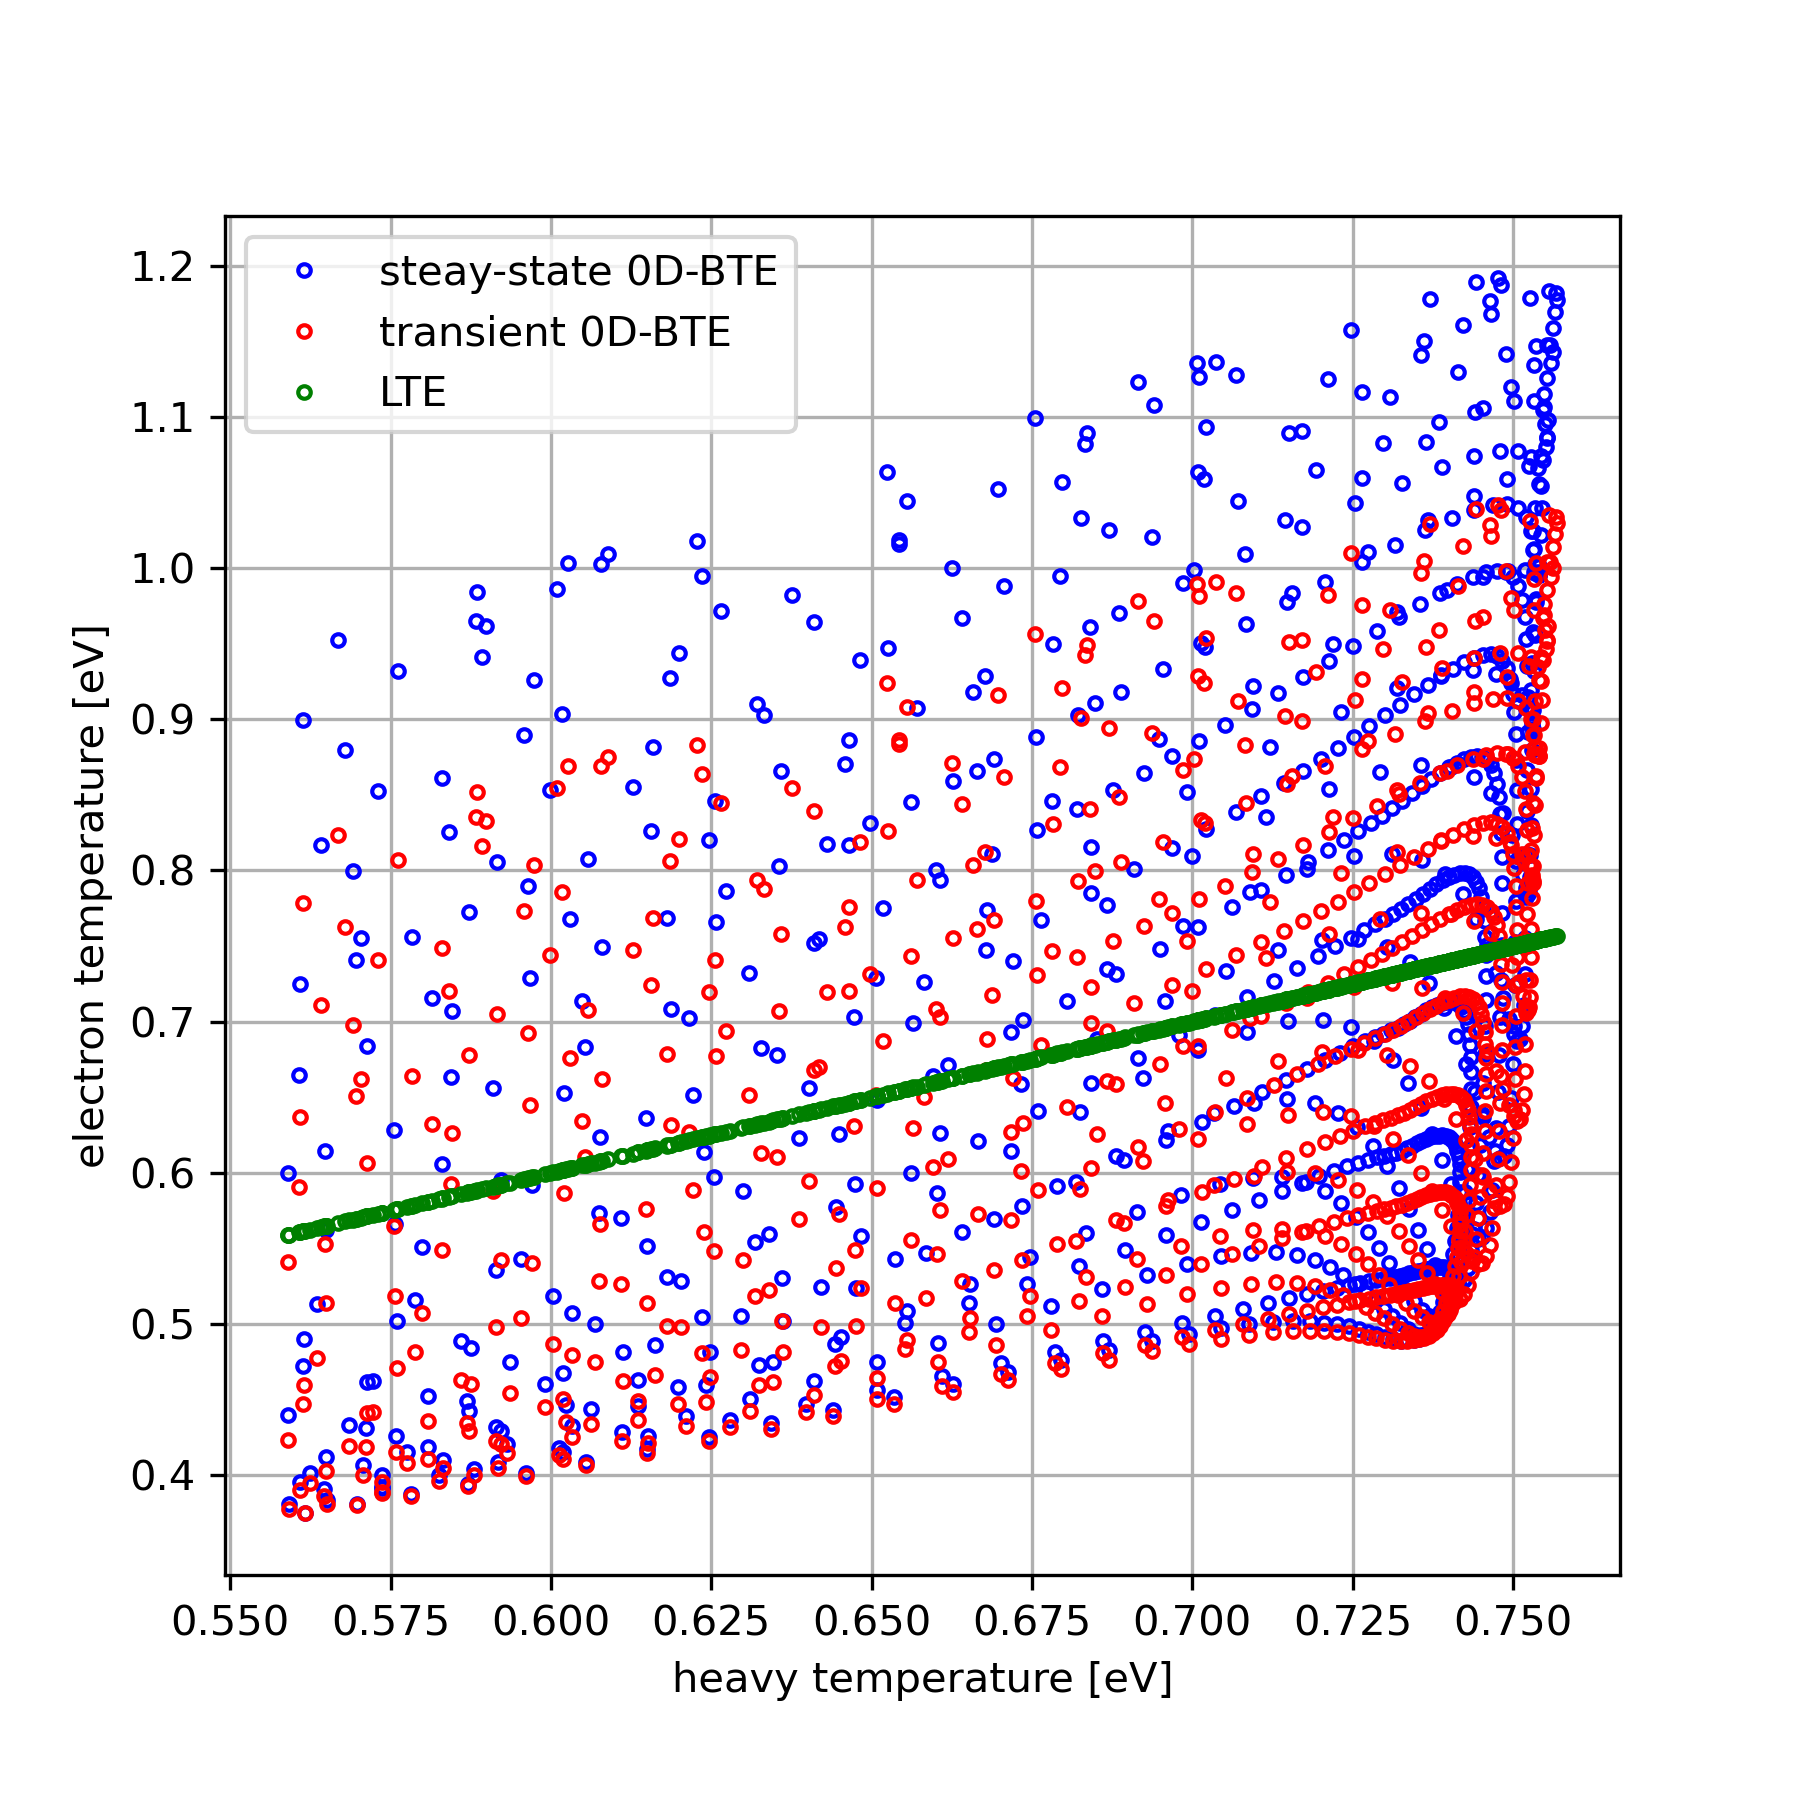
\includegraphics[width=0.48\textwidth]{te_vs_tg_tps_bte.png}
		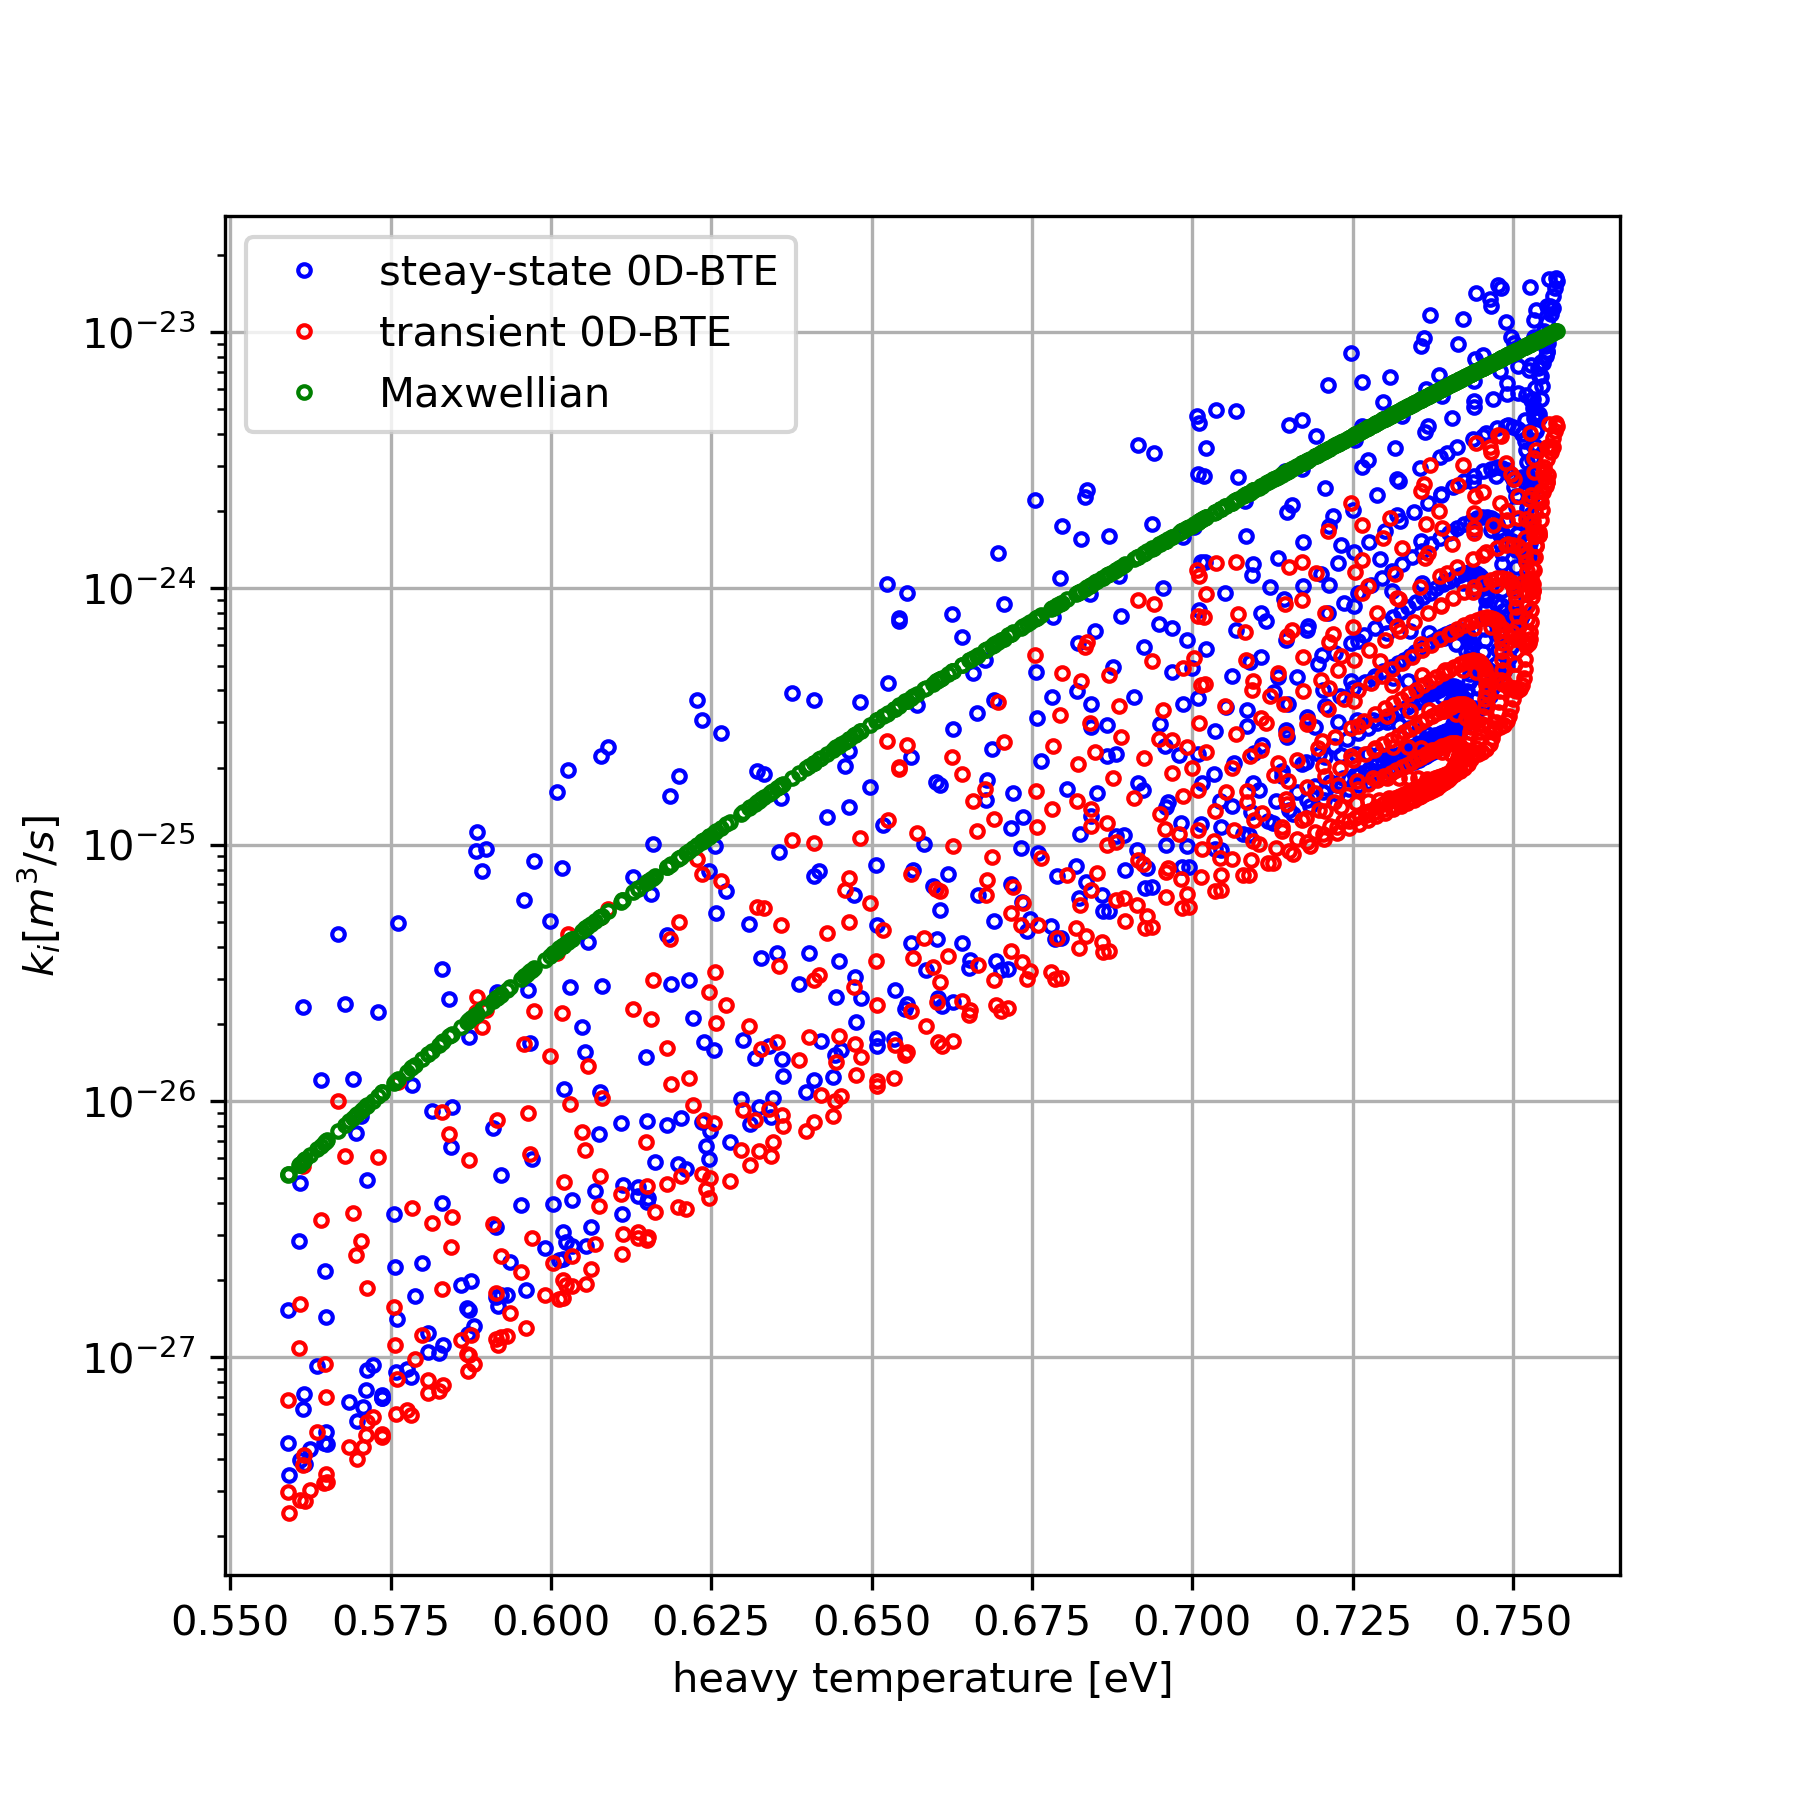
\includegraphics[width=0.48\textwidth]{rates_tps_bte.png}
	\end{figure}
\end{frame}

\begin{frame}
	\frametitle{Maxwellian vs. steady-state 0D-Boltzmann}
	\begin{figure}
		\begin{center}
			\includegraphics[width=1.05\textwidth]{tps_0d2v_ss.png}
		\end{center}
	\end{figure}
	\textbullet~ Relative errors for $k_i n_0 n_i$ 50\% compared to Maxwellian EEDF
\end{frame}

\begin{frame}
	\frametitle{Maxwellian vs. transient 0D-Boltzmann}
	\begin{figure}
		\begin{center}
			%\hspace{-0.6in}
			\includegraphics[width=1.05\textwidth]{tps_0d2v_ts.png}
		\end{center}
	\end{figure}
	\textbullet~ Relative errors for $k_i n_0 n_i$ 200\% compared to Maxwellian EEDF
\end{frame}


% \begin{frame}
% 	\frametitle{steady-state Vs. transient 0D-Boltzmann}
% 	% \begin{itemize}
% 	% 	%\item \textbf{A} : Assume LTE $T_e=T_g$ and $f_M(\vect{v}, t)=M_{T_e}(\vect{v})$ and $k_i^{M} = \mathcal{K}f_M$
% 	% 	\item \textbf{B} : Batched 0D-Boltzmann solver with static $\vect{E}$ , $k_i^{B} = \mathcal{K}f$ with weak-coupling
% 	% 	\item \textbf{C} : Batched 0D-Boltzmann solver with oscillatory $\vect{E}$ field with cycle averaged rates, $k_i^{C} = \mathcal{K}f$ with weak-coupling
% 	% \end{itemize}
% 	\begin{figure}
% 		\begin{center}
% 			%\hspace{-2.25in}
% 			%\vspace{-0.5in}
% 			\includegraphics[width=0.8\textwidth]{tps_0d2v_ts_vs_ss.png}
% 		\end{center}
% 	\end{figure}
% \end{frame}


% \begin{frame}
% 	\frametitle{Boltzmann equation}
% 	\begin{itemize}
% 		\item \textbf{Objective} : Enable accurate plasma simulations by solving the Boltzmann equation for electron distribution function.
% 		\item For a given electric field $\vect{E}$
% 		\begin{align}
% 			\partial_t f -\frac{\vect{E} q}{m} \cdot \nabla_{\vect{v }}f = C_{en}f + C_{ee}(f)
% 		\end{align}
% 		\item $C_{en}$ : electron-heavy collisions (i.e., elastic, ionization)
% 		\begin{itemize}
% 			\item Use LXCAT cross-section data 
% 			\item Linear in $f$
% 		\end{itemize} 
% 		\item $C_{ee}$ : electron-electron Columbic collisions 
% 		\begin{itemize}
% 			\item Modeled using Fokker-Plank equation with analytical cross-section
% 			\item Nonlinear in $f$
% 		\end{itemize}
% 		\item With $f$ we can compute electron kinetic coefficients, reaction rates and other QoIs. 
% 		%\item $C_{ei}$: electron-ion Columbic can be modeled similarly if needed
% 		%		\item Derived the steady state equation
% 		%		\begin{align}
% 			%			\textcolor{black!70}{\partial_t \hat{f} = -(u^T C \hat{f}) \hat{f} + (C+E)\hat{f} \text{ where } \hat{f}(\vect{v},t) = \frac{f(v,t)}{\myint_{R^3} f(\vect{v},t) \diff{\vect{v}}}}\\
% 			%			\textcolor{black!70}{\partial_t (\hat{f}) = 0 \ \ \  \Rightarrow} \ \ \  -(u^T C \hat{f}) \hat{f} + (C+E)\hat{f} =0  \text{ with } u^T \hat{f}-1=0
% 			%		\end{align}
% 	\end{itemize}
% \end{frame}

% \begin{frame}
% 	\frametitle{Discretization}
% 	\small
% 	\begin{itemize}
% 		\item Representation of $f\of{\vect{v},t} = \sum_{klm} f_{klm} \underbrace{\phi_k\of{v}}_{\text{B-Spline basis}} \underbrace{Y_{lm}\of{v_\theta, v_\phi}}_{\tiny\text{sph. harm.}}$ 
% %		\item Weak formulation
% %		$
% %		\displaystyle
% %		\quad
% %		\partial_t f - \frac{\vect{E} q}{m} \cdot \nabla_{\vect{v}}f = C(f)
% %		\quad $ \\
% %		$
% %		\displaystyle
% %		\quad
% %		\Rightarrow \quad
% %		\partial_t \myint_{R^3} f \phi\of{\vect{v}} \ud \vect{v} = 
% %		\myint_{R^3} C(f) \phi\of{\vect{v}} \ud \vect{v} + \myint_{R^3} \of{\frac{\vect{E} q}{m} \cdot \nabla_{\vect{v}} f} \phi(\vect{v}) \ud \vect{v}\text{ , } 
% %		\forall \phi(\vect{v})$
% 		\item Discretized system $\Rightarrow$
% 		$
% 		\displaystyle
% 		\quad
% 		\partial_t f  = C_{en}f + C_{ee}(f,f) + E A_v f
% 		$ where $C_{en}, A_v$ are matrices and $C_{ee}$ is a rank 3 tensor\\
% 		%\item In spatially homogeneous case (with isotropic scattering) azimuthal symmetry is preserved (i.e., 2 dimensions in v-space)
% 		\item Most cases can be resolved with 128 splines in radial direction with 2-spherical modes $\Rightarrow$ 256 DoFs in total
% 		%		\item Weak form of the collision operator (5d integral) \\
% 		%		$
% 		%		\displaystyle
% 		%		\quad 
% 		%		\myint_{R^3} C_{en} \phi\of{\vect{v}_e} \diff{\vect{v}_e} 
% 		%		=
% 		%		N \myint_{R^3} \myint_{S^2} 
% 		%		v\sigma(v,\vect{\omega})
% 		%		f_e\of{\vect{v}_e}
% 		%		\left(
% 		%		\psi\of{\vect{v}_e^\text{post}\of{\vect{v}_e, \vect{\omega}}} 
% 		%		- \psi\of{\vect{v}_e} 
% 		%		\right)
% 		%		\diff{\vect{v}_e} \diff{\vect{\omega}}
% 		%		$
% 		%		\item Isotropic scattering, azimuthal symmetry, and using spherical harmonics addition (1d integral)\\
% 		%		$
% 		%		\displaystyle
% 		%		\quad 
% 		%		C_{en}^{ql} 
% 		%		=
% 		%		N \myint_{0}^{\infty} 
% 		%		v^3\sigma(v)\delta_{ql}
% 		%		f_e^{l}\of{v}
% 		%		\left(
% 		%		\delta_{q0}\psi\of{v_e^\text{post}\of{v}} - \psi\of{v} 
% 		%		\right)
% 		%		\diff{v} 
% 		%		$ 
% 	\end{itemize}
% \end{frame}

% \begin{frame}
% 	\frametitle{Overview: TPS + 0D2V Boltzmann coupling}
% 	\begin{figure}
% 		\resizebox{0.9\textwidth}{!}{
% 			\centering
% 			\begin{tikzpicture}[block/.style={draw=black,thick, inner sep=2pt, rounded corners, minimum width=2cm, minimum height=1.2cm, fill=rightfooterorange,font={\small}}, shift=(current page.center)]
% 				\begin{scope}[yshift=10cm,xshift=5cm]
% 					\draw[lightgray]
% 					(current page.north) -- (current page.south)
% 					(current page.west)  -- (current page.east);
% 					\node[block] (A) at (-9, 3) {torch plasma simulator};
% 					\node[block] (B) at (0 , 6) {cross-section data};
% 					\node[block] (C) at (0.001 , 3.001) {0D2V-Boltzmann};
% 					\node[block] (D) at (0.002 , 0) {electron kinetic coefficients ($T_g, E/n_0, n_e/n_0, E$)};
% 					\draw [->,very thick] (B) -- node [text width=3cm, midway, above, align=center,xshift =-0.8cm] {with Maxwellian assumption $f = M_{T_e}(\vect{v})$} (A);\pause
% 					\draw [->,very thick] (B) -- node [text width=3cm, midway, above, align=center,xshift = 1.6cm, yshift=-0.5cm] {collision operator assembly} (C);
% 					\draw [->,very thick] (C) -- node [text width=3cm, midway, above, align=center, yshift=-0.5cm, xshift=1.2cm] {static E-field assumption} (D);
% 					\draw [->,very thick] (D) -- node [text width=3cm, midway, above, align=center,xshift =-1.2cm, yshift=-1.8cm] {$T_e$-based \\ interpolation for rates, kinetic coefficients} (A);\pause
% 					\draw [->,very thick,red] (A) to[bend left  = 8] node [text width=3cm, midway, above, align=center,yshift=0cm] {$T_g, E(x,t), n_e, n_0$} (C);
% 					\draw [->,very thick,red] (C) to[bend left  = 8] node [text width=3cm, midway, below, align=center,xshift=1.0cm] {rate coefficients, mobility, diffusion} (A);
% 				\end{scope}
% 		\end{tikzpicture}}
% 	\end{figure}
% \end{frame}

% \begin{frame}
% 	\frametitle{Methodology: TPS + 0D2V Boltzmann}
% 	\begin{itemize}
% 		\item Launch independent BTE solves for each spatial point roughly 256 DoF per grid point
% 		\item Challenges
% 		\begin{itemize}
% 			\item \textbf{computational cost}: Expensive to launch BTE solves for each spatial DoF 
% 			\item \textbf{grid truncation}: $v_{max} = \gamma \sqrt{\epsilon_{max}}$ v-space grid needs to be truncated depending on BTE input parameters
% 			\item \textbf{memory footprint}: Infeasible to have independent v-space grid for each spatial point
% 		\end{itemize}
% 		\item \textbf{p-coarsening}: Launch BTE solve for each TPS mesh cell 
% 		\item \textbf{Memory footprint}: Spatial points are clustered based on the approximate electron temperature ($T_e$), number of clusters can be specified by the user. Each cluster of points have the same v-space grid.
% 		\item \textbf{Grid truncation} : $T_e$ is also used to determine $v_{max}$
% 		\item For the TPS $T_e \approx$  0.02 eV to 0.8 eV
		
		
% %		Launch 0D2V BTE solves for each spatial gird point
% %		\item BTE require ~ 256 DoF per grid point
% %		\item One-way coupling
% %		\begin{itemize}
% %			\item Evolve the TPS solution till time-periodic steady-state
% %		\end{itemize}
% 	\end{itemize}
% \end{frame}

% \begin{frame}
% 	\frametitle{0D2V batched BTE solver}
% 	\begin{columns}
% 		\begin{column}{0.4\textwidth}
% 			\includegraphics[width=\columnwidth]{tps_input0.png}
% 		\end{column}
% 		\begin{column}{0.6\textwidth}
% 			For each cluster A
% 			\begin{itemize}
% 				\item Let $N_A$ be the number of spatial points
% 				\item Right-hand-side computation done by stacking BTE DoFs 
% 				\begin{align*}
% 					\underbrace{C}_{\text{v-space operator for cluster A}} \underbrace{\begin{bmatrix}
% 						\vdots & \vdots & \hdots &\vdots\\
% 						f_1    & f_2    & \hdots & f_{N_A} \\
% 						\vdots & \vdots & \hdots &\vdots
% 					\end{bmatrix}}_{\text{batched DoFs for cluster A}}
% 				\end{align*}
% 				\item \texttt{Numpy} and \texttt{Cupy} is used for efficient linear algebra computations in CPUs and GPUs
% 			\end{itemize}
% 		\end{column}
% 	\end{columns}
% \end{frame}


\begin{frame}
	\frametitle{Batched 0D-Boltzmann}
	\begin{itemize}
		\item For $N$ 0D-BTE solves, cluster points by input gas temperature. 
		\item Let $N_A$ be the number of points in cluster A
		\item Right-hand-side computation done by stacking BTE DoFs 
		\begin{align*}
			\underbrace{C_{en}, C_{ee}, A_{v}}_{\text{pre-computed v-space operator for cluster A}} \underbrace{\begin{bmatrix}
				\vdots & \vdots & \hdots &\vdots\\
				f_1    & f_2    & \hdots & f_{N_A} \\
				\vdots & \vdots & \hdots &\vdots
			\end{bmatrix}}_{\text{batched DoFs for cluster A}}
		\end{align*}
		%\item \texttt{Numpy} and \text{Cupy} is used for linear algebra computations
	\end{itemize}
	Boltzmann + Parla + MPI
	\begin{itemize}
		\item \textbf{Parla} is used for parallelization between clusters
		\item \textbf{MPI} is used for distributed memory parallelism
		\item 0D-BTE batched solver is integrated with TPS code
	\end{itemize}
\end{frame}

% \begin{frame}
% 	\frametitle{Software integration}
% 	\begin{itemize}
% 		\item \textbf{Plasma torch simulator (TPS)}: MFEM based discontinuous Galerkin discretization for the torch
% 		\begin{itemize}
% 			\item CPU, GPU support through MFEM library
% 			\item Python interface
% 		\end{itemize}
% 		\item \textbf{0D-space Boltzmann solver}
% 		\begin{itemize}
% 			%\item Galerkin discretization for the v-space
% 			\item Verified with Bolsig+ and PIC-DSMC codes
% 			\item Direct steady-state solution and fully-implicit time integrators for transient solutions
% 			%\item Python implementation
% 			\item CPU \& GPU support through \texttt{numpy} and \texttt{cupy}
% 		\end{itemize}
% 		\item \textbf{Parla}: Generic framework for task-based parallelism in Python
% 			\begin{itemize}
% 			\item Ability to handle fine grain tasks
% 			\item Support for CPU/GPU tasks with asynchronous kernel execution
% 			\item C/C++ based underlying task scheduler
% 			\end{itemize}
% 	\end{itemize}
% 	Current integration
% 	\begin{itemize}
% 		\item TPS + Python + MPI
% 		\item TPS + Boltzmann + Python + MPI + Parla
% 	\end{itemize}
	
% 	% \begin{itemize}
% 	% 	\item \textbf{Parla} is used for parallelization of clusters between GPUs on the same node
% 	% 	\item \textbf{MPI} is used for distributed memory parallelism
% 	% \end{itemize}
% \end{frame}

\begin{frame}
	\frametitle{TPS + Python + Boltzmann + Parla + MPI}
	\begin{figure}
		\centering
		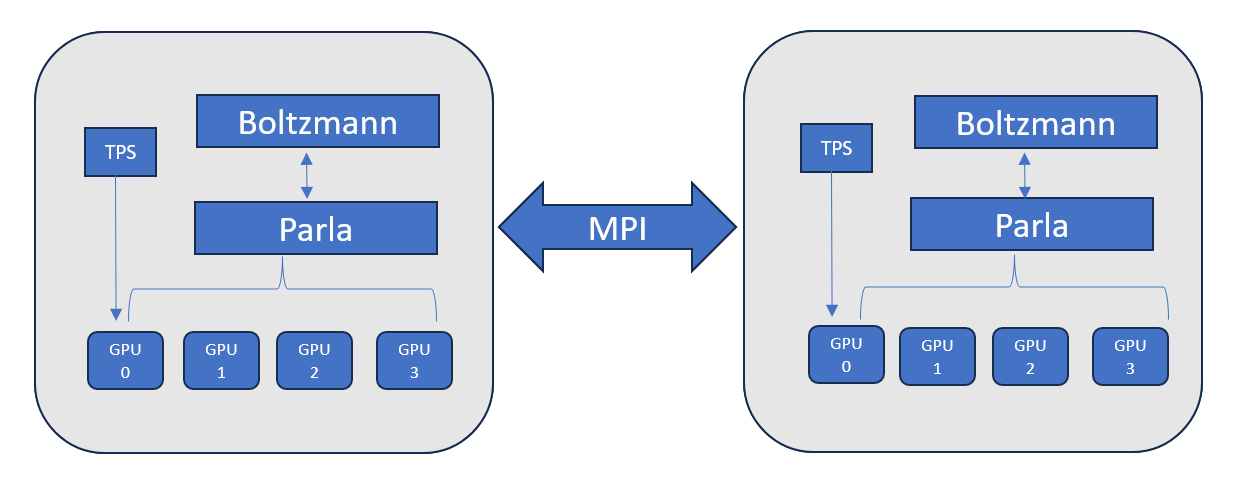
\includegraphics[width=0.8\textwidth]{software_integration.png}
	\end{figure}
	\begin{itemize}
		\item Information from Boltzmann to TPS is exchanged with interface class
		\item Spatial points are clustered using heavy temperature
		\item Different clusters $\rightarrow$ different $\epsilon_{max}$ truncation
		\item Parallelization between clusters via \textbf{Parla}
	\end{itemize}
\end{frame}

\begin{frame}[fragile]
	\frametitle{Scalability: TPS + 0D-Boltzmann}
%	TPS + 0D-Boltzmann problem setup
	\begin{itemize}
		\item spatial points = 7598, DoF per point = 256, Total DoFs $\approx$ 2M
		\item runtime for 200 implicit timesteps
		\item sclability study was performed in TACC's Lonestar 6 %$2\times 128$ AMD EPYC 7763 64-Core Processor with, 3-40GB Nvidia A100 GPU 
	\end{itemize}
	\begin{figure}
		\centering
		\begin{tikzpicture}
			\begin{axis}[
				width=8cm,
				height=5cm,
				ylabel={runtime (s)},
				xlabel={GPUs},
				symbolic x coords={3,6,12},
				xtick=data,
				grid=major
			]
			\addplot[-,mark=o,blue,thick] table[x={gpus}, y ={solve_max} ]{../ls6/tpp_0d2v_ss.dat};
		%\legend{Data1,Data2,Data3}
		\end{axis}
		\end{tikzpicture}
	\end{figure}
	\begin{itemize}
		\item 0D-Boltzmann grid setup $\approx$ 20s (independent of number of compute nodes)
		\item Parallel efficiency 78\%, 82\% $\rightarrow$ better load-balance with increasing partitions
	\end{itemize}
\end{frame}

\begin{frame}[fragile]
\frametitle{Strong coupling: TPS + 0D Boltzmann}
\begin{mintedbox}{python}%[break at=.8\textheight]
import libtps
from   bte_0d3v_batched import bte_0d3v_batched as BoltzmannSolver
comm = MPI.COMM_WORLD
tps = libtps.Tps(comm)
boltzmann = Boltzmann0D2VBactchedSolver(tps, comm)
interface = libtps.Tps2Boltzmann(tps)
it = 0
while it < max_iters:
    tps.solveStep()
    tps.push(interface)
    boltzmann.fetch(interface)
    boltzmann.solve()
    boltzmann.push(interface)
    tps.fetch(interface)
    it = it+1
\end{mintedbox}
\end{frame}

% \begin{frame}
% 	\frametitle{TPS + 0D2V Boltzmann weak coupling}
% 	\vspace{-0.2in}
% 	\begin{enumerate}
% 		\item Let $\vect{U}_0$ be the initial state for TPS (3-species, axisymmetric case)
% 		\item Evolve TPS solution until time-periodic $\vect{U}_{s}$ solution
% 		\item Extract TPS fields from $\vect{U}_s$ and start BTE solve with $E(\vect{x}, t) = E_x \cos(\omega t) + E_y \sin(\omega t)$, with Maxwellian initial conditions ($\vect{f}_0$)
% 		\item Evolve BTE solution $\vect{f}_0$ until time-periodic solutions $\vect{f}_s$
% 		\item Compute cycle-averaged reaction rates from $\vect{f}_s$ and compare with the rates coefficients used in the TPS code
% 	\end{enumerate}
% \pause
% \textbf{Problem setup}
% \begin{columns}
% 	\begin{column}{0.35\textwidth}

% 		\begin{itemize}
% 			\item TPS mesh elements 7598
% 			\item Number of spatial clusters 4
% 			\item DoFs per spatial point 256, i.e.,  2M DoFs total
% 			\item Number of timesteps 4000
% 			\item Number of GPUs 2 Nvidia A100
% 		\end{itemize}		
% 	\end{column}
% 	\begin{column}{0.7\textwidth}
% 		\begin{itemize}
% 			\item BTE grid setup time $\approx$ 29.3 s
% 			\item Assuming static E-field (direct steady-state solve) $\approx$ 8.07 s
% 			\item Cycle-averaged solution with time-integration (2 cycles, 4000 timesteps) $\approx$ 1314.0 s
% 		\end{itemize}
% 	\end{column}
% \end{columns}
% \end{frame}
% \begin{frame}
% 	\frametitle{TPS + 0D2V Boltzmann weak coupling}
% 	\begin{figure}
% 		\centering
% 		\includegraphics[width=0.5\textwidth]{initial_boltzmann_rxn_comparison.png}
% 	\end{figure}
% \end{frame}

% \begin{frame}
% 	\frametitle{TPS + 0D2V Boltzmann weak coupling}
% 	\vspace{-0.3in}
% 	\begin{figure}
% 		\centering
% 		\includegraphics[width=0.9\textwidth]{tps_bte_comparison1.png}
% 	\end{figure}
% \end{frame}
%\begin{frame}
%	\frametitle{0D-Space Boltzmann one-way coupling}
%	
%\end{frame}

\begin{frame}
	\frametitle{Conclusions}
	\begin{itemize}
		\item Observe significant errors between Maxwellian EEDF vs. 0D-Boltzmann for electrons %Solver with TPS + Boltzmann + Parla + MPI 
		\item Characterize $k_i$ model error sensitivity for torch QoIs
		\item Explore 1D, 2D space Boltzmann for torch 
		\item Detailed performance analysis for Batched Boltzmann
	\end{itemize}
	% \vspace{0.125in}
	% Ongoing Work
	% \begin{itemize}
	% 	\item Characterize sensitivity for electron kinetic coefficients to torch stability profiles
	% 	\item HPC \& performance for TPS + Boltzmann
	% 	\item 1D2V Boltzmann setup for glow discharge
	% \end{itemize}
	\pause
	\begin{center}
		Questions ? \\
		Thank You!
	\end{center}
\end{frame}
\end{document}
